Our algorithms can be seen in appendix \ref{app:algs}. All our searches will suffer from the fixed expansion order. Suppose the domain for $x_{j}$ is the singleton set $\set{v}$, and we assign $v$ to $x_i$, a peer of $x_j$, with $i<j$. Then we do not check the constraint $(i,j)$ until at depth $j$ even though it is very clear that $x_i$ can not be assigned $v$. This is fixed with our preprocessing as $v$ would be removed from $D_i$. It can also be made better by clever back jumping.

In Figure \ref{fig:exp1} we can see the Sudoku puzzles provided for benchmarking. The performance of our algorithms without and with arc-consistency can be seen in Table \ref{tab:exp1}, all of which produced a valid solution.

\begin{center}
    \begin{figure}[ht]
      \centering
      \def\scale{0.28}
      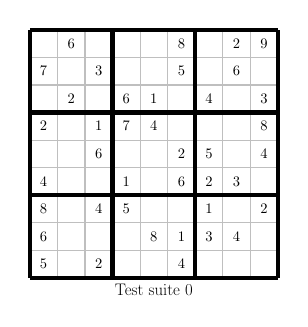
\begin{tikzpicture}[scale=\scale, every node/.style={scale=\scale}]
      \node[anchor=center,scale=1.5] at (1.5, 8.5) {$6$};
      \node[anchor=center,scale=1.5] at (5.5, 8.5) {$8$};
      \node[anchor=center,scale=1.5] at (7.5, 8.5) {$2$};
      \node[anchor=center,scale=1.5] at (8.5, 8.5) {$9$};
      \node[anchor=center,scale=1.5] at (0.5, 7.5) {$7$};
      \node[anchor=center,scale=1.5] at (2.5, 7.5) {$3$};
      \node[anchor=center,scale=1.5] at (5.5, 7.5) {$5$};
      \node[anchor=center,scale=1.5] at (7.5, 7.5) {$6$};
      \node[anchor=center,scale=1.5] at (1.5, 6.5) {$2$};
      \node[anchor=center,scale=1.5] at (3.5, 6.5) {$6$};
      \node[anchor=center,scale=1.5] at (4.5, 6.5) {$1$};
      \node[anchor=center,scale=1.5] at (6.5, 6.5) {$4$};
      \node[anchor=center,scale=1.5] at (8.5, 6.5) {$3$};
      \node[anchor=center,scale=1.5] at (0.5, 5.5) {$2$};
      \node[anchor=center,scale=1.5] at (2.5, 5.5) {$1$};
      \node[anchor=center,scale=1.5] at (3.5, 5.5) {$7$};
      \node[anchor=center,scale=1.5] at (4.5, 5.5) {$4$};
      \node[anchor=center,scale=1.5] at (8.5, 5.5) {$8$};
      \node[anchor=center,scale=1.5] at (2.5, 4.5) {$6$};
      \node[anchor=center,scale=1.5] at (5.5, 4.5) {$2$};
      \node[anchor=center,scale=1.5] at (6.5, 4.5) {$5$};
      \node[anchor=center,scale=1.5] at (8.5, 4.5) {$4$};
      \node[anchor=center,scale=1.5] at (0.5, 3.5) {$4$};
      \node[anchor=center,scale=1.5] at (3.5, 3.5) {$1$};
      \node[anchor=center,scale=1.5] at (5.5, 3.5) {$6$};
      \node[anchor=center,scale=1.5] at (6.5, 3.5) {$2$};
      \node[anchor=center,scale=1.5] at (7.5, 3.5) {$3$};
      \node[anchor=center,scale=1.5] at (0.5, 2.5) {$8$};
      \node[anchor=center,scale=1.5] at (2.5, 2.5) {$4$};
      \node[anchor=center,scale=1.5] at (3.5, 2.5) {$5$};
      \node[anchor=center,scale=1.5] at (6.5, 2.5) {$1$};
      \node[anchor=center,scale=1.5] at (8.5, 2.5) {$2$};
      \node[anchor=center,scale=1.5] at (0.5, 1.5) {$6$};
      \node[anchor=center,scale=1.5] at (4.5, 1.5) {$8$};
      \node[anchor=center,scale=1.5] at (5.5, 1.5) {$1$};
      \node[anchor=center,scale=1.5] at (6.5, 1.5) {$3$};
      \node[anchor=center,scale=1.5] at (7.5, 1.5) {$4$};
      \node[anchor=center,scale=1.5] at (0.5, 0.5) {$5$};
      \node[anchor=center,scale=1.5] at (2.5, 0.5) {$2$};
      \node[anchor=center,scale=1.5] at (5.5, 0.5) {$4$};
      \draw[gray!50] (0,0) grid (9,9);
      \draw[line width=0.55mm, scale=3] (0, 0) grid (3, 3);
      \draw (4.5,-.1) node[below] {\LARGE{Test suite 0}};
    \end{tikzpicture}
    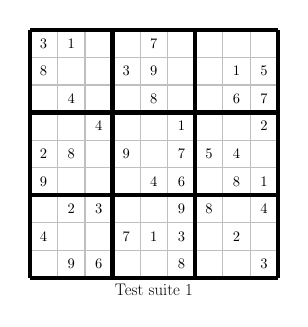
\begin{tikzpicture}[scale=\scale, every node/.style={scale=\scale}]
      \node[anchor=center,scale=1.5] at (0.5, 8.5) {$3$};
      \node[anchor=center,scale=1.5] at (1.5, 8.5) {$1$};
      \node[anchor=center,scale=1.5] at (4.5, 8.5) {$7$};
      \node[anchor=center,scale=1.5] at (0.5, 7.5) {$8$};
      \node[anchor=center,scale=1.5] at (3.5, 7.5) {$3$};
      \node[anchor=center,scale=1.5] at (4.5, 7.5) {$9$};
      \node[anchor=center,scale=1.5] at (7.5, 7.5) {$1$};
      \node[anchor=center,scale=1.5] at (8.5, 7.5) {$5$};
      \node[anchor=center,scale=1.5] at (1.5, 6.5) {$4$};
      \node[anchor=center,scale=1.5] at (4.5, 6.5) {$8$};
      \node[anchor=center,scale=1.5] at (7.5, 6.5) {$6$};
      \node[anchor=center,scale=1.5] at (8.5, 6.5) {$7$};
      \node[anchor=center,scale=1.5] at (2.5, 5.5) {$4$};
      \node[anchor=center,scale=1.5] at (5.5, 5.5) {$1$};
      \node[anchor=center,scale=1.5] at (8.5, 5.5) {$2$};
      \node[anchor=center,scale=1.5] at (0.5, 4.5) {$2$};
      \node[anchor=center,scale=1.5] at (1.5, 4.5) {$8$};
      \node[anchor=center,scale=1.5] at (3.5, 4.5) {$9$};
      \node[anchor=center,scale=1.5] at (5.5, 4.5) {$7$};
      \node[anchor=center,scale=1.5] at (6.5, 4.5) {$5$};
      \node[anchor=center,scale=1.5] at (7.5, 4.5) {$4$};
      \node[anchor=center,scale=1.5] at (0.5, 3.5) {$9$};
      \node[anchor=center,scale=1.5] at (4.5, 3.5) {$4$};
      \node[anchor=center,scale=1.5] at (5.5, 3.5) {$6$};
      \node[anchor=center,scale=1.5] at (7.5, 3.5) {$8$};
      \node[anchor=center,scale=1.5] at (8.5, 3.5) {$1$};
      \node[anchor=center,scale=1.5] at (1.5, 2.5) {$2$};
      \node[anchor=center,scale=1.5] at (2.5, 2.5) {$3$};
      \node[anchor=center,scale=1.5] at (5.5, 2.5) {$9$};
      \node[anchor=center,scale=1.5] at (6.5, 2.5) {$8$};
      \node[anchor=center,scale=1.5] at (8.5, 2.5) {$4$};
      \node[anchor=center,scale=1.5] at (0.5, 1.5) {$4$};
      \node[anchor=center,scale=1.5] at (3.5, 1.5) {$7$};
      \node[anchor=center,scale=1.5] at (4.5, 1.5) {$1$};
      \node[anchor=center,scale=1.5] at (5.5, 1.5) {$3$};
      \node[anchor=center,scale=1.5] at (7.5, 1.5) {$2$};
      \node[anchor=center,scale=1.5] at (1.5, 0.5) {$9$};
      \node[anchor=center,scale=1.5] at (2.5, 0.5) {$6$};
      \node[anchor=center,scale=1.5] at (5.5, 0.5) {$8$};
      \node[anchor=center,scale=1.5] at (8.5, 0.5) {$3$};
      \draw[gray!50] (0,0) grid (9,9);
      \draw[line width=0.55mm, scale=3] (0, 0) grid (3, 3);
      \draw (4.5,-.1) node[below] {\LARGE{Test suite 1}};
    \end{tikzpicture}
    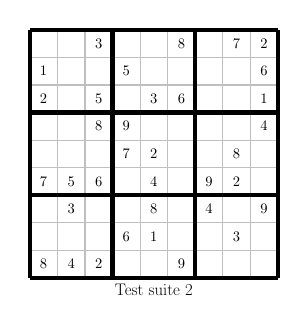
\begin{tikzpicture}[scale=\scale, every node/.style={scale=\scale}]
      \node[anchor=center,scale=1.5] at (2.5, 8.5) {$3$};
      \node[anchor=center,scale=1.5] at (5.5, 8.5) {$8$};
      \node[anchor=center,scale=1.5] at (7.5, 8.5) {$7$};
      \node[anchor=center,scale=1.5] at (8.5, 8.5) {$2$};
      \node[anchor=center,scale=1.5] at (0.5, 7.5) {$1$};
      \node[anchor=center,scale=1.5] at (3.5, 7.5) {$5$};
      \node[anchor=center,scale=1.5] at (8.5, 7.5) {$6$};
      \node[anchor=center,scale=1.5] at (0.5, 6.5) {$2$};
      \node[anchor=center,scale=1.5] at (2.5, 6.5) {$5$};
      \node[anchor=center,scale=1.5] at (4.5, 6.5) {$3$};
      \node[anchor=center,scale=1.5] at (5.5, 6.5) {$6$};
      \node[anchor=center,scale=1.5] at (8.5, 6.5) {$1$};
      \node[anchor=center,scale=1.5] at (2.5, 5.5) {$8$};
      \node[anchor=center,scale=1.5] at (3.5, 5.5) {$9$};
      \node[anchor=center,scale=1.5] at (8.5, 5.5) {$4$};
      \node[anchor=center,scale=1.5] at (3.5, 4.5) {$7$};
      \node[anchor=center,scale=1.5] at (4.5, 4.5) {$2$};
      \node[anchor=center,scale=1.5] at (7.5, 4.5) {$8$};
      \node[anchor=center,scale=1.5] at (0.5, 3.5) {$7$};
      \node[anchor=center,scale=1.5] at (1.5, 3.5) {$5$};
      \node[anchor=center,scale=1.5] at (2.5, 3.5) {$6$};
      \node[anchor=center,scale=1.5] at (4.5, 3.5) {$4$};
      \node[anchor=center,scale=1.5] at (6.5, 3.5) {$9$};
      \node[anchor=center,scale=1.5] at (7.5, 3.5) {$2$};
      \node[anchor=center,scale=1.5] at (1.5, 2.5) {$3$};
      \node[anchor=center,scale=1.5] at (4.5, 2.5) {$8$};
      \node[anchor=center,scale=1.5] at (6.5, 2.5) {$4$};
      \node[anchor=center,scale=1.5] at (8.5, 2.5) {$9$};
      \node[anchor=center,scale=1.5] at (3.5, 1.5) {$6$};
      \node[anchor=center,scale=1.5] at (4.5, 1.5) {$1$};
      \node[anchor=center,scale=1.5] at (7.5, 1.5) {$3$};
      \node[anchor=center,scale=1.5] at (0.5, 0.5) {$8$};
      \node[anchor=center,scale=1.5] at (1.5, 0.5) {$4$};
      \node[anchor=center,scale=1.5] at (2.5, 0.5) {$2$};
      \node[anchor=center,scale=1.5] at (5.5, 0.5) {$9$};
      \draw[gray!50] (0,0) grid (9,9);
      \draw[line width=0.55mm, scale=3] (0, 0) grid (3, 3);
      \draw (4.5,-.1) node[below] {\LARGE{Test suite 2}};
    \end{tikzpicture}
    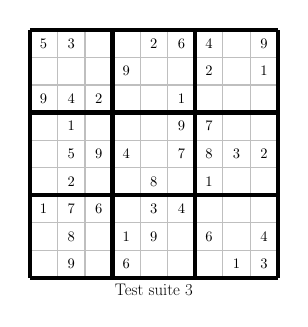
\begin{tikzpicture}[scale=\scale, every node/.style={scale=\scale}]
      \node[anchor=center,scale=1.5] at (0.5, 8.5) {$5$};
      \node[anchor=center,scale=1.5] at (1.5, 8.5) {$3$};
      \node[anchor=center,scale=1.5] at (4.5, 8.5) {$2$};
      \node[anchor=center,scale=1.5] at (5.5, 8.5) {$6$};
      \node[anchor=center,scale=1.5] at (6.5, 8.5) {$4$};
      \node[anchor=center,scale=1.5] at (8.5, 8.5) {$9$};
      \node[anchor=center,scale=1.5] at (3.5, 7.5) {$9$};
      \node[anchor=center,scale=1.5] at (6.5, 7.5) {$2$};
      \node[anchor=center,scale=1.5] at (8.5, 7.5) {$1$};
      \node[anchor=center,scale=1.5] at (0.5, 6.5) {$9$};
      \node[anchor=center,scale=1.5] at (1.5, 6.5) {$4$};
      \node[anchor=center,scale=1.5] at (2.5, 6.5) {$2$};
      \node[anchor=center,scale=1.5] at (5.5, 6.5) {$1$};
      \node[anchor=center,scale=1.5] at (1.5, 5.5) {$1$};
      \node[anchor=center,scale=1.5] at (5.5, 5.5) {$9$};
      \node[anchor=center,scale=1.5] at (6.5, 5.5) {$7$};
      \node[anchor=center,scale=1.5] at (1.5, 4.5) {$5$};
      \node[anchor=center,scale=1.5] at (2.5, 4.5) {$9$};
      \node[anchor=center,scale=1.5] at (3.5, 4.5) {$4$};
      \node[anchor=center,scale=1.5] at (5.5, 4.5) {$7$};
      \node[anchor=center,scale=1.5] at (6.5, 4.5) {$8$};
      \node[anchor=center,scale=1.5] at (7.5, 4.5) {$3$};
      \node[anchor=center,scale=1.5] at (8.5, 4.5) {$2$};
      \node[anchor=center,scale=1.5] at (1.5, 3.5) {$2$};
      \node[anchor=center,scale=1.5] at (4.5, 3.5) {$8$};
      \node[anchor=center,scale=1.5] at (6.5, 3.5) {$1$};
      \node[anchor=center,scale=1.5] at (0.5, 2.5) {$1$};
      \node[anchor=center,scale=1.5] at (1.5, 2.5) {$7$};
      \node[anchor=center,scale=1.5] at (2.5, 2.5) {$6$};
      \node[anchor=center,scale=1.5] at (4.5, 2.5) {$3$};
      \node[anchor=center,scale=1.5] at (5.5, 2.5) {$4$};
      \node[anchor=center,scale=1.5] at (1.5, 1.5) {$8$};
      \node[anchor=center,scale=1.5] at (3.5, 1.5) {$1$};
      \node[anchor=center,scale=1.5] at (4.5, 1.5) {$9$};
      \node[anchor=center,scale=1.5] at (6.5, 1.5) {$6$};
      \node[anchor=center,scale=1.5] at (8.5, 1.5) {$4$};
      \node[anchor=center,scale=1.5] at (1.5, 0.5) {$9$};
      \node[anchor=center,scale=1.5] at (3.5, 0.5) {$6$};
      \node[anchor=center,scale=1.5] at (7.5, 0.5) {$1$};
      \node[anchor=center,scale=1.5] at (8.5, 0.5) {$3$};
      \draw[gray!50] (0,0) grid (9,9);
      \draw[line width=0.55mm, scale=3] (0, 0) grid (3, 3);
      \draw (4.5,-.1) node[below] {\LARGE{Test suite 3}};
    \end{tikzpicture}
    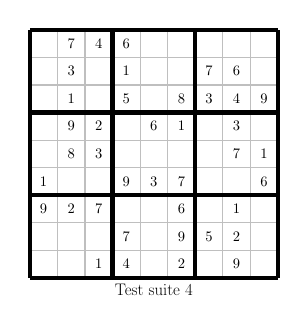
\begin{tikzpicture}[scale=\scale, every node/.style={scale=\scale}]
      \node[anchor=center,scale=1.5] at (1.5, 8.5) {$7$};
      \node[anchor=center,scale=1.5] at (2.5, 8.5) {$4$};
      \node[anchor=center,scale=1.5] at (3.5, 8.5) {$6$};
      \node[anchor=center,scale=1.5] at (1.5, 7.5) {$3$};
      \node[anchor=center,scale=1.5] at (3.5, 7.5) {$1$};
      \node[anchor=center,scale=1.5] at (6.5, 7.5) {$7$};
      \node[anchor=center,scale=1.5] at (7.5, 7.5) {$6$};
      \node[anchor=center,scale=1.5] at (1.5, 6.5) {$1$};
      \node[anchor=center,scale=1.5] at (3.5, 6.5) {$5$};
      \node[anchor=center,scale=1.5] at (5.5, 6.5) {$8$};
      \node[anchor=center,scale=1.5] at (6.5, 6.5) {$3$};
      \node[anchor=center,scale=1.5] at (7.5, 6.5) {$4$};
      \node[anchor=center,scale=1.5] at (8.5, 6.5) {$9$};
      \node[anchor=center,scale=1.5] at (1.5, 5.5) {$9$};
      \node[anchor=center,scale=1.5] at (2.5, 5.5) {$2$};
      \node[anchor=center,scale=1.5] at (4.5, 5.5) {$6$};
      \node[anchor=center,scale=1.5] at (5.5, 5.5) {$1$};
      \node[anchor=center,scale=1.5] at (7.5, 5.5) {$3$};
      \node[anchor=center,scale=1.5] at (1.5, 4.5) {$8$};
      \node[anchor=center,scale=1.5] at (2.5, 4.5) {$3$};
      \node[anchor=center,scale=1.5] at (7.5, 4.5) {$7$};
      \node[anchor=center,scale=1.5] at (8.5, 4.5) {$1$};
      \node[anchor=center,scale=1.5] at (0.5, 3.5) {$1$};
      \node[anchor=center,scale=1.5] at (3.5, 3.5) {$9$};
      \node[anchor=center,scale=1.5] at (4.5, 3.5) {$3$};
      \node[anchor=center,scale=1.5] at (5.5, 3.5) {$7$};
      \node[anchor=center,scale=1.5] at (8.5, 3.5) {$6$};
      \node[anchor=center,scale=1.5] at (0.5, 2.5) {$9$};
      \node[anchor=center,scale=1.5] at (1.5, 2.5) {$2$};
      \node[anchor=center,scale=1.5] at (2.5, 2.5) {$7$};
      \node[anchor=center,scale=1.5] at (5.5, 2.5) {$6$};
      \node[anchor=center,scale=1.5] at (7.5, 2.5) {$1$};
      \node[anchor=center,scale=1.5] at (3.5, 1.5) {$7$};
      \node[anchor=center,scale=1.5] at (5.5, 1.5) {$9$};
      \node[anchor=center,scale=1.5] at (6.5, 1.5) {$5$};
      \node[anchor=center,scale=1.5] at (7.5, 1.5) {$2$};
      \node[anchor=center,scale=1.5] at (2.5, 0.5) {$1$};
      \node[anchor=center,scale=1.5] at (3.5, 0.5) {$4$};
      \node[anchor=center,scale=1.5] at (5.5, 0.5) {$2$};
      \node[anchor=center,scale=1.5] at (7.5, 0.5) {$9$};
      \draw[gray!50] (0,0) grid (9,9);
      \draw[line width=0.55mm, scale=3] (0, 0) grid (3, 3);
      \draw (4.5,-.1) node[below] {\LARGE{Test suite 4}};
    \end{tikzpicture}

    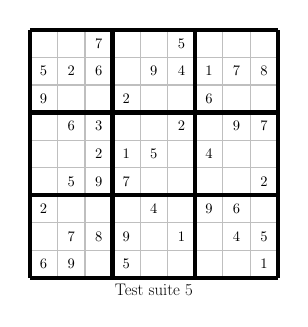
\begin{tikzpicture}[scale=\scale, every node/.style={scale=\scale}]
      \node[anchor=center,scale=1.5] at (2.5, 8.5) {$7$};
      \node[anchor=center,scale=1.5] at (5.5, 8.5) {$5$};
      \node[anchor=center,scale=1.5] at (0.5, 7.5) {$5$};
      \node[anchor=center,scale=1.5] at (1.5, 7.5) {$2$};
      \node[anchor=center,scale=1.5] at (2.5, 7.5) {$6$};
      \node[anchor=center,scale=1.5] at (4.5, 7.5) {$9$};
      \node[anchor=center,scale=1.5] at (5.5, 7.5) {$4$};
      \node[anchor=center,scale=1.5] at (6.5, 7.5) {$1$};
      \node[anchor=center,scale=1.5] at (7.5, 7.5) {$7$};
      \node[anchor=center,scale=1.5] at (8.5, 7.5) {$8$};
      \node[anchor=center,scale=1.5] at (0.5, 6.5) {$9$};
      \node[anchor=center,scale=1.5] at (3.5, 6.5) {$2$};
      \node[anchor=center,scale=1.5] at (6.5, 6.5) {$6$};
      \node[anchor=center,scale=1.5] at (1.5, 5.5) {$6$};
      \node[anchor=center,scale=1.5] at (2.5, 5.5) {$3$};
      \node[anchor=center,scale=1.5] at (5.5, 5.5) {$2$};
      \node[anchor=center,scale=1.5] at (7.5, 5.5) {$9$};
      \node[anchor=center,scale=1.5] at (8.5, 5.5) {$7$};
      \node[anchor=center,scale=1.5] at (2.5, 4.5) {$2$};
      \node[anchor=center,scale=1.5] at (3.5, 4.5) {$1$};
      \node[anchor=center,scale=1.5] at (4.5, 4.5) {$5$};
      \node[anchor=center,scale=1.5] at (6.5, 4.5) {$4$};
      \node[anchor=center,scale=1.5] at (1.5, 3.5) {$5$};
      \node[anchor=center,scale=1.5] at (2.5, 3.5) {$9$};
      \node[anchor=center,scale=1.5] at (3.5, 3.5) {$7$};
      \node[anchor=center,scale=1.5] at (8.5, 3.5) {$2$};
      \node[anchor=center,scale=1.5] at (0.5, 2.5) {$2$};
      \node[anchor=center,scale=1.5] at (4.5, 2.5) {$4$};
      \node[anchor=center,scale=1.5] at (6.5, 2.5) {$9$};
      \node[anchor=center,scale=1.5] at (7.5, 2.5) {$6$};
      \node[anchor=center,scale=1.5] at (1.5, 1.5) {$7$};
      \node[anchor=center,scale=1.5] at (2.5, 1.5) {$8$};
      \node[anchor=center,scale=1.5] at (3.5, 1.5) {$9$};
      \node[anchor=center,scale=1.5] at (5.5, 1.5) {$1$};
      \node[anchor=center,scale=1.5] at (7.5, 1.5) {$4$};
      \node[anchor=center,scale=1.5] at (8.5, 1.5) {$5$};
      \node[anchor=center,scale=1.5] at (0.5, 0.5) {$6$};
      \node[anchor=center,scale=1.5] at (1.5, 0.5) {$9$};
      \node[anchor=center,scale=1.5] at (3.5, 0.5) {$5$};
      \node[anchor=center,scale=1.5] at (8.5, 0.5) {$1$};
      \draw[gray!50] (0,0) grid (9,9);
      \draw[line width=0.55mm, scale=3] (0, 0) grid (3, 3);
      \draw (4.5,-.1) node[below] {\LARGE{Test suite 5}};
    \end{tikzpicture}
    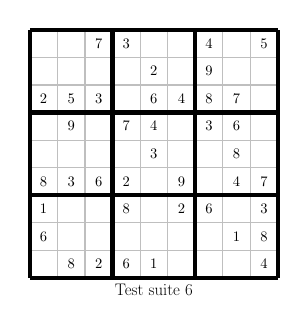
\begin{tikzpicture}[scale=\scale, every node/.style={scale=\scale}]
      \node[anchor=center,scale=1.5] at (2.5, 8.5) {$7$};
      \node[anchor=center,scale=1.5] at (3.5, 8.5) {$3$};
      \node[anchor=center,scale=1.5] at (6.5, 8.5) {$4$};
      \node[anchor=center,scale=1.5] at (8.5, 8.5) {$5$};
      \node[anchor=center,scale=1.5] at (4.5, 7.5) {$2$};
      \node[anchor=center,scale=1.5] at (6.5, 7.5) {$9$};
      \node[anchor=center,scale=1.5] at (0.5, 6.5) {$2$};
      \node[anchor=center,scale=1.5] at (1.5, 6.5) {$5$};
      \node[anchor=center,scale=1.5] at (2.5, 6.5) {$3$};
      \node[anchor=center,scale=1.5] at (4.5, 6.5) {$6$};
      \node[anchor=center,scale=1.5] at (5.5, 6.5) {$4$};
      \node[anchor=center,scale=1.5] at (6.5, 6.5) {$8$};
      \node[anchor=center,scale=1.5] at (7.5, 6.5) {$7$};
      \node[anchor=center,scale=1.5] at (1.5, 5.5) {$9$};
      \node[anchor=center,scale=1.5] at (3.5, 5.5) {$7$};
      \node[anchor=center,scale=1.5] at (4.5, 5.5) {$4$};
      \node[anchor=center,scale=1.5] at (6.5, 5.5) {$3$};
      \node[anchor=center,scale=1.5] at (7.5, 5.5) {$6$};
      \node[anchor=center,scale=1.5] at (4.5, 4.5) {$3$};
      \node[anchor=center,scale=1.5] at (7.5, 4.5) {$8$};
      \node[anchor=center,scale=1.5] at (0.5, 3.5) {$8$};
      \node[anchor=center,scale=1.5] at (1.5, 3.5) {$3$};
      \node[anchor=center,scale=1.5] at (2.5, 3.5) {$6$};
      \node[anchor=center,scale=1.5] at (3.5, 3.5) {$2$};
      \node[anchor=center,scale=1.5] at (5.5, 3.5) {$9$};
      \node[anchor=center,scale=1.5] at (7.5, 3.5) {$4$};
      \node[anchor=center,scale=1.5] at (8.5, 3.5) {$7$};
      \node[anchor=center,scale=1.5] at (0.5, 2.5) {$1$};
      \node[anchor=center,scale=1.5] at (3.5, 2.5) {$8$};
      \node[anchor=center,scale=1.5] at (5.5, 2.5) {$2$};
      \node[anchor=center,scale=1.5] at (6.5, 2.5) {$6$};
      \node[anchor=center,scale=1.5] at (8.5, 2.5) {$3$};
      \node[anchor=center,scale=1.5] at (0.5, 1.5) {$6$};
      \node[anchor=center,scale=1.5] at (7.5, 1.5) {$1$};
      \node[anchor=center,scale=1.5] at (8.5, 1.5) {$8$};
      \node[anchor=center,scale=1.5] at (1.5, 0.5) {$8$};
      \node[anchor=center,scale=1.5] at (2.5, 0.5) {$2$};
      \node[anchor=center,scale=1.5] at (3.5, 0.5) {$6$};
      \node[anchor=center,scale=1.5] at (4.5, 0.5) {$1$};
      \node[anchor=center,scale=1.5] at (8.5, 0.5) {$4$};
      \draw[gray!50] (0,0) grid (9,9);
      \draw[line width=0.55mm, scale=3] (0, 0) grid (3, 3);
      \draw (4.5,-.1) node[below] {\LARGE{Test suite 6}};
    \end{tikzpicture}
    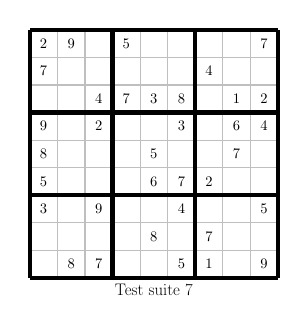
\begin{tikzpicture}[scale=\scale, every node/.style={scale=\scale}]
      \node[anchor=center,scale=1.5] at (0.5, 8.5) {$2$};
      \node[anchor=center,scale=1.5] at (1.5, 8.5) {$9$};
      \node[anchor=center,scale=1.5] at (3.5, 8.5) {$5$};
      \node[anchor=center,scale=1.5] at (8.5, 8.5) {$7$};
      \node[anchor=center,scale=1.5] at (0.5, 7.5) {$7$};
      \node[anchor=center,scale=1.5] at (6.5, 7.5) {$4$};
      \node[anchor=center,scale=1.5] at (2.5, 6.5) {$4$};
      \node[anchor=center,scale=1.5] at (3.5, 6.5) {$7$};
      \node[anchor=center,scale=1.5] at (4.5, 6.5) {$3$};
      \node[anchor=center,scale=1.5] at (5.5, 6.5) {$8$};
      \node[anchor=center,scale=1.5] at (7.5, 6.5) {$1$};
      \node[anchor=center,scale=1.5] at (8.5, 6.5) {$2$};
      \node[anchor=center,scale=1.5] at (0.5, 5.5) {$9$};
      \node[anchor=center,scale=1.5] at (2.5, 5.5) {$2$};
      \node[anchor=center,scale=1.5] at (5.5, 5.5) {$3$};
      \node[anchor=center,scale=1.5] at (7.5, 5.5) {$6$};
      \node[anchor=center,scale=1.5] at (8.5, 5.5) {$4$};
      \node[anchor=center,scale=1.5] at (0.5, 4.5) {$8$};
      \node[anchor=center,scale=1.5] at (4.5, 4.5) {$5$};
      \node[anchor=center,scale=1.5] at (7.5, 4.5) {$7$};
      \node[anchor=center,scale=1.5] at (0.5, 3.5) {$5$};
      \node[anchor=center,scale=1.5] at (4.5, 3.5) {$6$};
      \node[anchor=center,scale=1.5] at (5.5, 3.5) {$7$};
      \node[anchor=center,scale=1.5] at (6.5, 3.5) {$2$};
      \node[anchor=center,scale=1.5] at (0.5, 2.5) {$3$};
      \node[anchor=center,scale=1.5] at (2.5, 2.5) {$9$};
      \node[anchor=center,scale=1.5] at (5.5, 2.5) {$4$};
      \node[anchor=center,scale=1.5] at (8.5, 2.5) {$5$};
      \node[anchor=center,scale=1.5] at (4.5, 1.5) {$8$};
      \node[anchor=center,scale=1.5] at (6.5, 1.5) {$7$};
      \node[anchor=center,scale=1.5] at (1.5, 0.5) {$8$};
      \node[anchor=center,scale=1.5] at (2.5, 0.5) {$7$};
      \node[anchor=center,scale=1.5] at (5.5, 0.5) {$5$};
      \node[anchor=center,scale=1.5] at (6.5, 0.5) {$1$};
      \node[anchor=center,scale=1.5] at (8.5, 0.5) {$9$};
      \draw[gray!50] (0,0) grid (9,9);
      \draw[line width=0.55mm, scale=3] (0, 0) grid (3, 3);
      \draw (4.5,-.1) node[below] {\LARGE{Test suite 7}};
    \end{tikzpicture}
    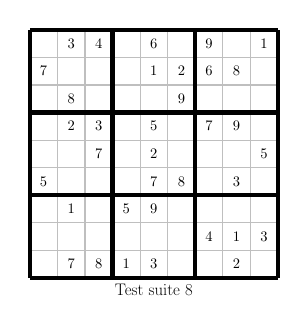
\begin{tikzpicture}[scale=\scale, every node/.style={scale=\scale}]
      \node[anchor=center,scale=1.5] at (1.5, 8.5) {$3$};
      \node[anchor=center,scale=1.5] at (2.5, 8.5) {$4$};
      \node[anchor=center,scale=1.5] at (4.5, 8.5) {$6$};
      \node[anchor=center,scale=1.5] at (6.5, 8.5) {$9$};
      \node[anchor=center,scale=1.5] at (8.5, 8.5) {$1$};
      \node[anchor=center,scale=1.5] at (0.5, 7.5) {$7$};
      \node[anchor=center,scale=1.5] at (4.5, 7.5) {$1$};
      \node[anchor=center,scale=1.5] at (5.5, 7.5) {$2$};
      \node[anchor=center,scale=1.5] at (6.5, 7.5) {$6$};
      \node[anchor=center,scale=1.5] at (7.5, 7.5) {$8$};
      \node[anchor=center,scale=1.5] at (1.5, 6.5) {$8$};
      \node[anchor=center,scale=1.5] at (5.5, 6.5) {$9$};
      \node[anchor=center,scale=1.5] at (1.5, 5.5) {$2$};
      \node[anchor=center,scale=1.5] at (2.5, 5.5) {$3$};
      \node[anchor=center,scale=1.5] at (4.5, 5.5) {$5$};
      \node[anchor=center,scale=1.5] at (6.5, 5.5) {$7$};
      \node[anchor=center,scale=1.5] at (7.5, 5.5) {$9$};
      \node[anchor=center,scale=1.5] at (2.5, 4.5) {$7$};
      \node[anchor=center,scale=1.5] at (4.5, 4.5) {$2$};
      \node[anchor=center,scale=1.5] at (8.5, 4.5) {$5$};
      \node[anchor=center,scale=1.5] at (0.5, 3.5) {$5$};
      \node[anchor=center,scale=1.5] at (4.5, 3.5) {$7$};
      \node[anchor=center,scale=1.5] at (5.5, 3.5) {$8$};
      \node[anchor=center,scale=1.5] at (7.5, 3.5) {$3$};
      \node[anchor=center,scale=1.5] at (1.5, 2.5) {$1$};
      \node[anchor=center,scale=1.5] at (3.5, 2.5) {$5$};
      \node[anchor=center,scale=1.5] at (4.5, 2.5) {$9$};
      \node[anchor=center,scale=1.5] at (6.5, 1.5) {$4$};
      \node[anchor=center,scale=1.5] at (7.5, 1.5) {$1$};
      \node[anchor=center,scale=1.5] at (8.5, 1.5) {$3$};
      \node[anchor=center,scale=1.5] at (1.5, 0.5) {$7$};
      \node[anchor=center,scale=1.5] at (2.5, 0.5) {$8$};
      \node[anchor=center,scale=1.5] at (3.5, 0.5) {$1$};
      \node[anchor=center,scale=1.5] at (4.5, 0.5) {$3$};
      \node[anchor=center,scale=1.5] at (7.5, 0.5) {$2$};
      \draw[gray!50] (0,0) grid (9,9);
      \draw[line width=0.55mm, scale=3] (0, 0) grid (3, 3);
      \draw (4.5,-.1) node[below] {\LARGE{Test suite 8}};
    \end{tikzpicture}
    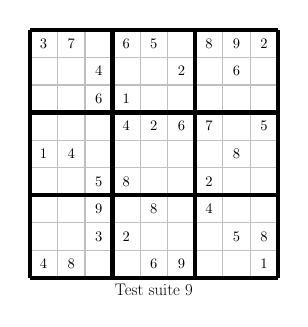
\begin{tikzpicture}[scale=\scale, every node/.style={scale=\scale}]
      \node[anchor=center,scale=1.5] at (0.5, 8.5) {$3$};
      \node[anchor=center,scale=1.5] at (1.5, 8.5) {$7$};
      \node[anchor=center,scale=1.5] at (3.5, 8.5) {$6$};
      \node[anchor=center,scale=1.5] at (4.5, 8.5) {$5$};
      \node[anchor=center,scale=1.5] at (6.5, 8.5) {$8$};
      \node[anchor=center,scale=1.5] at (7.5, 8.5) {$9$};
      \node[anchor=center,scale=1.5] at (8.5, 8.5) {$2$};
      \node[anchor=center,scale=1.5] at (2.5, 7.5) {$4$};
      \node[anchor=center,scale=1.5] at (5.5, 7.5) {$2$};
      \node[anchor=center,scale=1.5] at (7.5, 7.5) {$6$};
      \node[anchor=center,scale=1.5] at (2.5, 6.5) {$6$};
      \node[anchor=center,scale=1.5] at (3.5, 6.5) {$1$};
      \node[anchor=center,scale=1.5] at (3.5, 5.5) {$4$};
      \node[anchor=center,scale=1.5] at (4.5, 5.5) {$2$};
      \node[anchor=center,scale=1.5] at (5.5, 5.5) {$6$};
      \node[anchor=center,scale=1.5] at (6.5, 5.5) {$7$};
      \node[anchor=center,scale=1.5] at (8.5, 5.5) {$5$};
      \node[anchor=center,scale=1.5] at (0.5, 4.5) {$1$};
      \node[anchor=center,scale=1.5] at (1.5, 4.5) {$4$};
      \node[anchor=center,scale=1.5] at (7.5, 4.5) {$8$};
      \node[anchor=center,scale=1.5] at (2.5, 3.5) {$5$};
      \node[anchor=center,scale=1.5] at (3.5, 3.5) {$8$};
      \node[anchor=center,scale=1.5] at (6.5, 3.5) {$2$};
      \node[anchor=center,scale=1.5] at (2.5, 2.5) {$9$};
      \node[anchor=center,scale=1.5] at (4.5, 2.5) {$8$};
      \node[anchor=center,scale=1.5] at (6.5, 2.5) {$4$};
      \node[anchor=center,scale=1.5] at (2.5, 1.5) {$3$};
      \node[anchor=center,scale=1.5] at (3.5, 1.5) {$2$};
      \node[anchor=center,scale=1.5] at (7.5, 1.5) {$5$};
      \node[anchor=center,scale=1.5] at (8.5, 1.5) {$8$};
      \node[anchor=center,scale=1.5] at (0.5, 0.5) {$4$};
      \node[anchor=center,scale=1.5] at (1.5, 0.5) {$8$};
      \node[anchor=center,scale=1.5] at (4.5, 0.5) {$6$};
      \node[anchor=center,scale=1.5] at (5.5, 0.5) {$9$};
      \node[anchor=center,scale=1.5] at (8.5, 0.5) {$1$};
      \draw[gray!50] (0,0) grid (9,9);
      \draw[line width=0.55mm, scale=3] (0, 0) grid (3, 3);
      \draw (4.5,-.1) node[below] {\LARGE{Test suite 9}};
    \end{tikzpicture}

    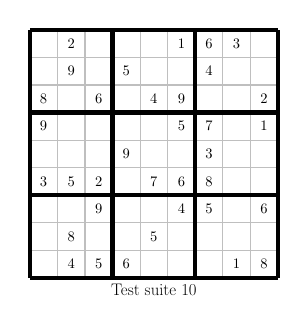
\begin{tikzpicture}[scale=\scale, every node/.style={scale=\scale}]
      \node[anchor=center,scale=1.5] at (1.5, 8.5) {$2$};
      \node[anchor=center,scale=1.5] at (5.5, 8.5) {$1$};
      \node[anchor=center,scale=1.5] at (6.5, 8.5) {$6$};
      \node[anchor=center,scale=1.5] at (7.5, 8.5) {$3$};
      \node[anchor=center,scale=1.5] at (1.5, 7.5) {$9$};
      \node[anchor=center,scale=1.5] at (3.5, 7.5) {$5$};
      \node[anchor=center,scale=1.5] at (6.5, 7.5) {$4$};
      \node[anchor=center,scale=1.5] at (0.5, 6.5) {$8$};
      \node[anchor=center,scale=1.5] at (2.5, 6.5) {$6$};
      \node[anchor=center,scale=1.5] at (4.5, 6.5) {$4$};
      \node[anchor=center,scale=1.5] at (5.5, 6.5) {$9$};
      \node[anchor=center,scale=1.5] at (8.5, 6.5) {$2$};
      \node[anchor=center,scale=1.5] at (0.5, 5.5) {$9$};
      \node[anchor=center,scale=1.5] at (5.5, 5.5) {$5$};
      \node[anchor=center,scale=1.5] at (6.5, 5.5) {$7$};
      \node[anchor=center,scale=1.5] at (8.5, 5.5) {$1$};
      \node[anchor=center,scale=1.5] at (3.5, 4.5) {$9$};
      \node[anchor=center,scale=1.5] at (6.5, 4.5) {$3$};
      \node[anchor=center,scale=1.5] at (0.5, 3.5) {$3$};
      \node[anchor=center,scale=1.5] at (1.5, 3.5) {$5$};
      \node[anchor=center,scale=1.5] at (2.5, 3.5) {$2$};
      \node[anchor=center,scale=1.5] at (4.5, 3.5) {$7$};
      \node[anchor=center,scale=1.5] at (5.5, 3.5) {$6$};
      \node[anchor=center,scale=1.5] at (6.5, 3.5) {$8$};
      \node[anchor=center,scale=1.5] at (2.5, 2.5) {$9$};
      \node[anchor=center,scale=1.5] at (5.5, 2.5) {$4$};
      \node[anchor=center,scale=1.5] at (6.5, 2.5) {$5$};
      \node[anchor=center,scale=1.5] at (8.5, 2.5) {$6$};
      \node[anchor=center,scale=1.5] at (1.5, 1.5) {$8$};
      \node[anchor=center,scale=1.5] at (4.5, 1.5) {$5$};
      \node[anchor=center,scale=1.5] at (1.5, 0.5) {$4$};
      \node[anchor=center,scale=1.5] at (2.5, 0.5) {$5$};
      \node[anchor=center,scale=1.5] at (3.5, 0.5) {$6$};
      \node[anchor=center,scale=1.5] at (7.5, 0.5) {$1$};
      \node[anchor=center,scale=1.5] at (8.5, 0.5) {$8$};
      \draw[gray!50] (0,0) grid (9,9);
      \draw[line width=0.55mm, scale=3] (0, 0) grid (3, 3);
      \draw (4.5,-.1) node[below] {\LARGE{Test suite 10}};
    \end{tikzpicture}
    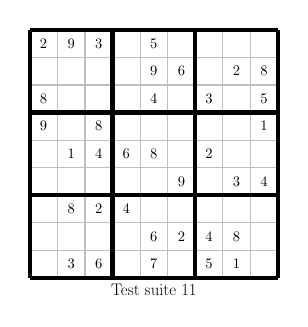
\begin{tikzpicture}[scale=\scale, every node/.style={scale=\scale}]
      \node[anchor=center,scale=1.5] at (0.5, 8.5) {$2$};
      \node[anchor=center,scale=1.5] at (1.5, 8.5) {$9$};
      \node[anchor=center,scale=1.5] at (2.5, 8.5) {$3$};
      \node[anchor=center,scale=1.5] at (4.5, 8.5) {$5$};
      \node[anchor=center,scale=1.5] at (4.5, 7.5) {$9$};
      \node[anchor=center,scale=1.5] at (5.5, 7.5) {$6$};
      \node[anchor=center,scale=1.5] at (7.5, 7.5) {$2$};
      \node[anchor=center,scale=1.5] at (8.5, 7.5) {$8$};
      \node[anchor=center,scale=1.5] at (0.5, 6.5) {$8$};
      \node[anchor=center,scale=1.5] at (4.5, 6.5) {$4$};
      \node[anchor=center,scale=1.5] at (6.5, 6.5) {$3$};
      \node[anchor=center,scale=1.5] at (8.5, 6.5) {$5$};
      \node[anchor=center,scale=1.5] at (0.5, 5.5) {$9$};
      \node[anchor=center,scale=1.5] at (2.5, 5.5) {$8$};
      \node[anchor=center,scale=1.5] at (8.5, 5.5) {$1$};
      \node[anchor=center,scale=1.5] at (1.5, 4.5) {$1$};
      \node[anchor=center,scale=1.5] at (2.5, 4.5) {$4$};
      \node[anchor=center,scale=1.5] at (3.5, 4.5) {$6$};
      \node[anchor=center,scale=1.5] at (4.5, 4.5) {$8$};
      \node[anchor=center,scale=1.5] at (6.5, 4.5) {$2$};
      \node[anchor=center,scale=1.5] at (5.5, 3.5) {$9$};
      \node[anchor=center,scale=1.5] at (7.5, 3.5) {$3$};
      \node[anchor=center,scale=1.5] at (8.5, 3.5) {$4$};
      \node[anchor=center,scale=1.5] at (1.5, 2.5) {$8$};
      \node[anchor=center,scale=1.5] at (2.5, 2.5) {$2$};
      \node[anchor=center,scale=1.5] at (3.5, 2.5) {$4$};
      \node[anchor=center,scale=1.5] at (4.5, 1.5) {$6$};
      \node[anchor=center,scale=1.5] at (5.5, 1.5) {$2$};
      \node[anchor=center,scale=1.5] at (6.5, 1.5) {$4$};
      \node[anchor=center,scale=1.5] at (7.5, 1.5) {$8$};
      \node[anchor=center,scale=1.5] at (1.5, 0.5) {$3$};
      \node[anchor=center,scale=1.5] at (2.5, 0.5) {$6$};
      \node[anchor=center,scale=1.5] at (4.5, 0.5) {$7$};
      \node[anchor=center,scale=1.5] at (6.5, 0.5) {$5$};
      \node[anchor=center,scale=1.5] at (7.5, 0.5) {$1$};
      \draw[gray!50] (0,0) grid (9,9);
      \draw[line width=0.55mm, scale=3] (0, 0) grid (3, 3);
      \draw (4.5,-.1) node[below] {\LARGE{Test suite 11}};
    \end{tikzpicture}
    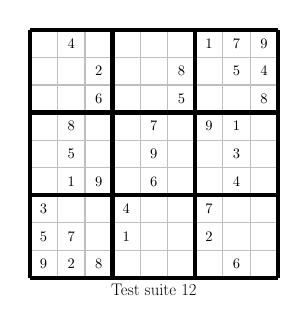
\begin{tikzpicture}[scale=\scale, every node/.style={scale=\scale}]
      \node[anchor=center,scale=1.5] at (1.5, 8.5) {$4$};
      \node[anchor=center,scale=1.5] at (6.5, 8.5) {$1$};
      \node[anchor=center,scale=1.5] at (7.5, 8.5) {$7$};
      \node[anchor=center,scale=1.5] at (8.5, 8.5) {$9$};
      \node[anchor=center,scale=1.5] at (2.5, 7.5) {$2$};
      \node[anchor=center,scale=1.5] at (5.5, 7.5) {$8$};
      \node[anchor=center,scale=1.5] at (7.5, 7.5) {$5$};
      \node[anchor=center,scale=1.5] at (8.5, 7.5) {$4$};
      \node[anchor=center,scale=1.5] at (2.5, 6.5) {$6$};
      \node[anchor=center,scale=1.5] at (5.5, 6.5) {$5$};
      \node[anchor=center,scale=1.5] at (8.5, 6.5) {$8$};
      \node[anchor=center,scale=1.5] at (1.5, 5.5) {$8$};
      \node[anchor=center,scale=1.5] at (4.5, 5.5) {$7$};
      \node[anchor=center,scale=1.5] at (6.5, 5.5) {$9$};
      \node[anchor=center,scale=1.5] at (7.5, 5.5) {$1$};
      \node[anchor=center,scale=1.5] at (1.5, 4.5) {$5$};
      \node[anchor=center,scale=1.5] at (4.5, 4.5) {$9$};
      \node[anchor=center,scale=1.5] at (7.5, 4.5) {$3$};
      \node[anchor=center,scale=1.5] at (1.5, 3.5) {$1$};
      \node[anchor=center,scale=1.5] at (2.5, 3.5) {$9$};
      \node[anchor=center,scale=1.5] at (4.5, 3.5) {$6$};
      \node[anchor=center,scale=1.5] at (7.5, 3.5) {$4$};
      \node[anchor=center,scale=1.5] at (0.5, 2.5) {$3$};
      \node[anchor=center,scale=1.5] at (3.5, 2.5) {$4$};
      \node[anchor=center,scale=1.5] at (6.5, 2.5) {$7$};
      \node[anchor=center,scale=1.5] at (0.5, 1.5) {$5$};
      \node[anchor=center,scale=1.5] at (1.5, 1.5) {$7$};
      \node[anchor=center,scale=1.5] at (3.5, 1.5) {$1$};
      \node[anchor=center,scale=1.5] at (6.5, 1.5) {$2$};
      \node[anchor=center,scale=1.5] at (0.5, 0.5) {$9$};
      \node[anchor=center,scale=1.5] at (1.5, 0.5) {$2$};
      \node[anchor=center,scale=1.5] at (2.5, 0.5) {$8$};
      \node[anchor=center,scale=1.5] at (7.5, 0.5) {$6$};
      \draw[gray!50] (0,0) grid (9,9);
      \draw[line width=0.55mm, scale=3] (0, 0) grid (3, 3);
      \draw (4.5,-.1) node[below] {\LARGE{Test suite 12}};
    \end{tikzpicture}
    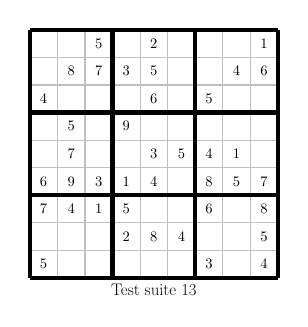
\begin{tikzpicture}[scale=\scale, every node/.style={scale=\scale}]
      \node[anchor=center,scale=1.5] at (2.5, 8.5) {$5$};
      \node[anchor=center,scale=1.5] at (4.5, 8.5) {$2$};
      \node[anchor=center,scale=1.5] at (8.5, 8.5) {$1$};
      \node[anchor=center,scale=1.5] at (1.5, 7.5) {$8$};
      \node[anchor=center,scale=1.5] at (2.5, 7.5) {$7$};
      \node[anchor=center,scale=1.5] at (3.5, 7.5) {$3$};
      \node[anchor=center,scale=1.5] at (4.5, 7.5) {$5$};
      \node[anchor=center,scale=1.5] at (7.5, 7.5) {$4$};
      \node[anchor=center,scale=1.5] at (8.5, 7.5) {$6$};
      \node[anchor=center,scale=1.5] at (0.5, 6.5) {$4$};
      \node[anchor=center,scale=1.5] at (4.5, 6.5) {$6$};
      \node[anchor=center,scale=1.5] at (6.5, 6.5) {$5$};
      \node[anchor=center,scale=1.5] at (1.5, 5.5) {$5$};
      \node[anchor=center,scale=1.5] at (3.5, 5.5) {$9$};
      \node[anchor=center,scale=1.5] at (1.5, 4.5) {$7$};
      \node[anchor=center,scale=1.5] at (4.5, 4.5) {$3$};
      \node[anchor=center,scale=1.5] at (5.5, 4.5) {$5$};
      \node[anchor=center,scale=1.5] at (6.5, 4.5) {$4$};
      \node[anchor=center,scale=1.5] at (7.5, 4.5) {$1$};
      \node[anchor=center,scale=1.5] at (0.5, 3.5) {$6$};
      \node[anchor=center,scale=1.5] at (1.5, 3.5) {$9$};
      \node[anchor=center,scale=1.5] at (2.5, 3.5) {$3$};
      \node[anchor=center,scale=1.5] at (3.5, 3.5) {$1$};
      \node[anchor=center,scale=1.5] at (4.5, 3.5) {$4$};
      \node[anchor=center,scale=1.5] at (6.5, 3.5) {$8$};
      \node[anchor=center,scale=1.5] at (7.5, 3.5) {$5$};
      \node[anchor=center,scale=1.5] at (8.5, 3.5) {$7$};
      \node[anchor=center,scale=1.5] at (0.5, 2.5) {$7$};
      \node[anchor=center,scale=1.5] at (1.5, 2.5) {$4$};
      \node[anchor=center,scale=1.5] at (2.5, 2.5) {$1$};
      \node[anchor=center,scale=1.5] at (3.5, 2.5) {$5$};
      \node[anchor=center,scale=1.5] at (6.5, 2.5) {$6$};
      \node[anchor=center,scale=1.5] at (8.5, 2.5) {$8$};
      \node[anchor=center,scale=1.5] at (3.5, 1.5) {$2$};
      \node[anchor=center,scale=1.5] at (4.5, 1.5) {$8$};
      \node[anchor=center,scale=1.5] at (5.5, 1.5) {$4$};
      \node[anchor=center,scale=1.5] at (8.5, 1.5) {$5$};
      \node[anchor=center,scale=1.5] at (0.5, 0.5) {$5$};
      \node[anchor=center,scale=1.5] at (6.5, 0.5) {$3$};
      \node[anchor=center,scale=1.5] at (8.5, 0.5) {$4$};
      \draw[gray!50] (0,0) grid (9,9);
      \draw[line width=0.55mm, scale=3] (0, 0) grid (3, 3);
      \draw (4.5,-.1) node[below] {\LARGE{Test suite 13}};
    \end{tikzpicture}
    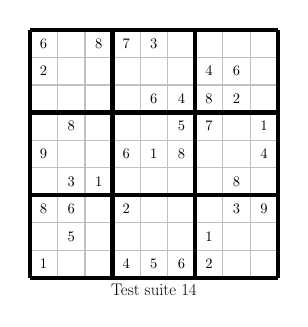
\begin{tikzpicture}[scale=\scale, every node/.style={scale=\scale}]
      \node[anchor=center,scale=1.5] at (0.5, 8.5) {$6$};
      \node[anchor=center,scale=1.5] at (2.5, 8.5) {$8$};
      \node[anchor=center,scale=1.5] at (3.5, 8.5) {$7$};
      \node[anchor=center,scale=1.5] at (4.5, 8.5) {$3$};
      \node[anchor=center,scale=1.5] at (0.5, 7.5) {$2$};
      \node[anchor=center,scale=1.5] at (6.5, 7.5) {$4$};
      \node[anchor=center,scale=1.5] at (7.5, 7.5) {$6$};
      \node[anchor=center,scale=1.5] at (4.5, 6.5) {$6$};
      \node[anchor=center,scale=1.5] at (5.5, 6.5) {$4$};
      \node[anchor=center,scale=1.5] at (6.5, 6.5) {$8$};
      \node[anchor=center,scale=1.5] at (7.5, 6.5) {$2$};
      \node[anchor=center,scale=1.5] at (1.5, 5.5) {$8$};
      \node[anchor=center,scale=1.5] at (5.5, 5.5) {$5$};
      \node[anchor=center,scale=1.5] at (6.5, 5.5) {$7$};
      \node[anchor=center,scale=1.5] at (8.5, 5.5) {$1$};
      \node[anchor=center,scale=1.5] at (0.5, 4.5) {$9$};
      \node[anchor=center,scale=1.5] at (3.5, 4.5) {$6$};
      \node[anchor=center,scale=1.5] at (4.5, 4.5) {$1$};
      \node[anchor=center,scale=1.5] at (5.5, 4.5) {$8$};
      \node[anchor=center,scale=1.5] at (8.5, 4.5) {$4$};
      \node[anchor=center,scale=1.5] at (1.5, 3.5) {$3$};
      \node[anchor=center,scale=1.5] at (2.5, 3.5) {$1$};
      \node[anchor=center,scale=1.5] at (7.5, 3.5) {$8$};
      \node[anchor=center,scale=1.5] at (0.5, 2.5) {$8$};
      \node[anchor=center,scale=1.5] at (1.5, 2.5) {$6$};
      \node[anchor=center,scale=1.5] at (3.5, 2.5) {$2$};
      \node[anchor=center,scale=1.5] at (7.5, 2.5) {$3$};
      \node[anchor=center,scale=1.5] at (8.5, 2.5) {$9$};
      \node[anchor=center,scale=1.5] at (1.5, 1.5) {$5$};
      \node[anchor=center,scale=1.5] at (6.5, 1.5) {$1$};
      \node[anchor=center,scale=1.5] at (0.5, 0.5) {$1$};
      \node[anchor=center,scale=1.5] at (3.5, 0.5) {$4$};
      \node[anchor=center,scale=1.5] at (4.5, 0.5) {$5$};
      \node[anchor=center,scale=1.5] at (5.5, 0.5) {$6$};
      \node[anchor=center,scale=1.5] at (6.5, 0.5) {$2$};
      \draw[gray!50] (0,0) grid (9,9);
      \draw[line width=0.55mm, scale=3] (0, 0) grid (3, 3);
      \draw (4.5,-.1) node[below] {\LARGE{Test suite 14}};
    \end{tikzpicture}

    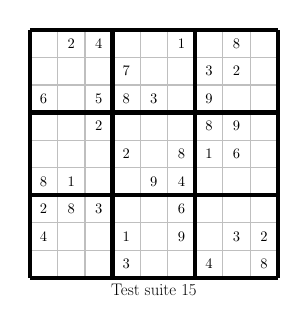
\begin{tikzpicture}[scale=\scale, every node/.style={scale=\scale}]
      \node[anchor=center,scale=1.5] at (1.5, 8.5) {$2$};
      \node[anchor=center,scale=1.5] at (2.5, 8.5) {$4$};
      \node[anchor=center,scale=1.5] at (5.5, 8.5) {$1$};
      \node[anchor=center,scale=1.5] at (7.5, 8.5) {$8$};
      \node[anchor=center,scale=1.5] at (3.5, 7.5) {$7$};
      \node[anchor=center,scale=1.5] at (6.5, 7.5) {$3$};
      \node[anchor=center,scale=1.5] at (7.5, 7.5) {$2$};
      \node[anchor=center,scale=1.5] at (0.5, 6.5) {$6$};
      \node[anchor=center,scale=1.5] at (2.5, 6.5) {$5$};
      \node[anchor=center,scale=1.5] at (3.5, 6.5) {$8$};
      \node[anchor=center,scale=1.5] at (4.5, 6.5) {$3$};
      \node[anchor=center,scale=1.5] at (6.5, 6.5) {$9$};
      \node[anchor=center,scale=1.5] at (2.5, 5.5) {$2$};
      \node[anchor=center,scale=1.5] at (6.5, 5.5) {$8$};
      \node[anchor=center,scale=1.5] at (7.5, 5.5) {$9$};
      \node[anchor=center,scale=1.5] at (3.5, 4.5) {$2$};
      \node[anchor=center,scale=1.5] at (5.5, 4.5) {$8$};
      \node[anchor=center,scale=1.5] at (6.5, 4.5) {$1$};
      \node[anchor=center,scale=1.5] at (7.5, 4.5) {$6$};
      \node[anchor=center,scale=1.5] at (0.5, 3.5) {$8$};
      \node[anchor=center,scale=1.5] at (1.5, 3.5) {$1$};
      \node[anchor=center,scale=1.5] at (4.5, 3.5) {$9$};
      \node[anchor=center,scale=1.5] at (5.5, 3.5) {$4$};
      \node[anchor=center,scale=1.5] at (0.5, 2.5) {$2$};
      \node[anchor=center,scale=1.5] at (1.5, 2.5) {$8$};
      \node[anchor=center,scale=1.5] at (2.5, 2.5) {$3$};
      \node[anchor=center,scale=1.5] at (5.5, 2.5) {$6$};
      \node[anchor=center,scale=1.5] at (0.5, 1.5) {$4$};
      \node[anchor=center,scale=1.5] at (3.5, 1.5) {$1$};
      \node[anchor=center,scale=1.5] at (5.5, 1.5) {$9$};
      \node[anchor=center,scale=1.5] at (7.5, 1.5) {$3$};
      \node[anchor=center,scale=1.5] at (8.5, 1.5) {$2$};
      \node[anchor=center,scale=1.5] at (3.5, 0.5) {$3$};
      \node[anchor=center,scale=1.5] at (6.5, 0.5) {$4$};
      \node[anchor=center,scale=1.5] at (8.5, 0.5) {$8$};
      \draw[gray!50] (0,0) grid (9,9);
      \draw[line width=0.55mm, scale=3] (0, 0) grid (3, 3);
      \draw (4.5,-.1) node[below] {\LARGE{Test suite 15}};
    \end{tikzpicture}
    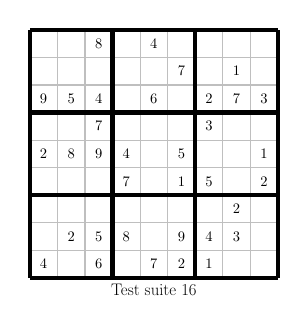
\begin{tikzpicture}[scale=\scale, every node/.style={scale=\scale}]
      \node[anchor=center,scale=1.5] at (2.5, 8.5) {$8$};
      \node[anchor=center,scale=1.5] at (4.5, 8.5) {$4$};
      \node[anchor=center,scale=1.5] at (5.5, 7.5) {$7$};
      \node[anchor=center,scale=1.5] at (7.5, 7.5) {$1$};
      \node[anchor=center,scale=1.5] at (0.5, 6.5) {$9$};
      \node[anchor=center,scale=1.5] at (1.5, 6.5) {$5$};
      \node[anchor=center,scale=1.5] at (2.5, 6.5) {$4$};
      \node[anchor=center,scale=1.5] at (4.5, 6.5) {$6$};
      \node[anchor=center,scale=1.5] at (6.5, 6.5) {$2$};
      \node[anchor=center,scale=1.5] at (7.5, 6.5) {$7$};
      \node[anchor=center,scale=1.5] at (8.5, 6.5) {$3$};
      \node[anchor=center,scale=1.5] at (2.5, 5.5) {$7$};
      \node[anchor=center,scale=1.5] at (6.5, 5.5) {$3$};
      \node[anchor=center,scale=1.5] at (0.5, 4.5) {$2$};
      \node[anchor=center,scale=1.5] at (1.5, 4.5) {$8$};
      \node[anchor=center,scale=1.5] at (2.5, 4.5) {$9$};
      \node[anchor=center,scale=1.5] at (3.5, 4.5) {$4$};
      \node[anchor=center,scale=1.5] at (5.5, 4.5) {$5$};
      \node[anchor=center,scale=1.5] at (8.5, 4.5) {$1$};
      \node[anchor=center,scale=1.5] at (3.5, 3.5) {$7$};
      \node[anchor=center,scale=1.5] at (5.5, 3.5) {$1$};
      \node[anchor=center,scale=1.5] at (6.5, 3.5) {$5$};
      \node[anchor=center,scale=1.5] at (8.5, 3.5) {$2$};
      \node[anchor=center,scale=1.5] at (7.5, 2.5) {$2$};
      \node[anchor=center,scale=1.5] at (1.5, 1.5) {$2$};
      \node[anchor=center,scale=1.5] at (2.5, 1.5) {$5$};
      \node[anchor=center,scale=1.5] at (3.5, 1.5) {$8$};
      \node[anchor=center,scale=1.5] at (5.5, 1.5) {$9$};
      \node[anchor=center,scale=1.5] at (6.5, 1.5) {$4$};
      \node[anchor=center,scale=1.5] at (7.5, 1.5) {$3$};
      \node[anchor=center,scale=1.5] at (0.5, 0.5) {$4$};
      \node[anchor=center,scale=1.5] at (2.5, 0.5) {$6$};
      \node[anchor=center,scale=1.5] at (4.5, 0.5) {$7$};
      \node[anchor=center,scale=1.5] at (5.5, 0.5) {$2$};
      \node[anchor=center,scale=1.5] at (6.5, 0.5) {$1$};
      \draw[gray!50] (0,0) grid (9,9);
      \draw[line width=0.55mm, scale=3] (0, 0) grid (3, 3);
      \draw (4.5,-.1) node[below] {\LARGE{Test suite 16}};
    \end{tikzpicture}
    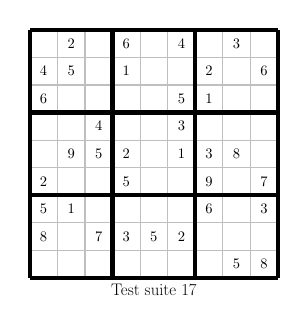
\begin{tikzpicture}[scale=\scale, every node/.style={scale=\scale}]
      \node[anchor=center,scale=1.5] at (1.5, 8.5) {$2$};
      \node[anchor=center,scale=1.5] at (3.5, 8.5) {$6$};
      \node[anchor=center,scale=1.5] at (5.5, 8.5) {$4$};
      \node[anchor=center,scale=1.5] at (7.5, 8.5) {$3$};
      \node[anchor=center,scale=1.5] at (0.5, 7.5) {$4$};
      \node[anchor=center,scale=1.5] at (1.5, 7.5) {$5$};
      \node[anchor=center,scale=1.5] at (3.5, 7.5) {$1$};
      \node[anchor=center,scale=1.5] at (6.5, 7.5) {$2$};
      \node[anchor=center,scale=1.5] at (8.5, 7.5) {$6$};
      \node[anchor=center,scale=1.5] at (0.5, 6.5) {$6$};
      \node[anchor=center,scale=1.5] at (5.5, 6.5) {$5$};
      \node[anchor=center,scale=1.5] at (6.5, 6.5) {$1$};
      \node[anchor=center,scale=1.5] at (2.5, 5.5) {$4$};
      \node[anchor=center,scale=1.5] at (5.5, 5.5) {$3$};
      \node[anchor=center,scale=1.5] at (1.5, 4.5) {$9$};
      \node[anchor=center,scale=1.5] at (2.5, 4.5) {$5$};
      \node[anchor=center,scale=1.5] at (3.5, 4.5) {$2$};
      \node[anchor=center,scale=1.5] at (5.5, 4.5) {$1$};
      \node[anchor=center,scale=1.5] at (6.5, 4.5) {$3$};
      \node[anchor=center,scale=1.5] at (7.5, 4.5) {$8$};
      \node[anchor=center,scale=1.5] at (0.5, 3.5) {$2$};
      \node[anchor=center,scale=1.5] at (3.5, 3.5) {$5$};
      \node[anchor=center,scale=1.5] at (6.5, 3.5) {$9$};
      \node[anchor=center,scale=1.5] at (8.5, 3.5) {$7$};
      \node[anchor=center,scale=1.5] at (0.5, 2.5) {$5$};
      \node[anchor=center,scale=1.5] at (1.5, 2.5) {$1$};
      \node[anchor=center,scale=1.5] at (6.5, 2.5) {$6$};
      \node[anchor=center,scale=1.5] at (8.5, 2.5) {$3$};
      \node[anchor=center,scale=1.5] at (0.5, 1.5) {$8$};
      \node[anchor=center,scale=1.5] at (2.5, 1.5) {$7$};
      \node[anchor=center,scale=1.5] at (3.5, 1.5) {$3$};
      \node[anchor=center,scale=1.5] at (4.5, 1.5) {$5$};
      \node[anchor=center,scale=1.5] at (5.5, 1.5) {$2$};
      \node[anchor=center,scale=1.5] at (7.5, 0.5) {$5$};
      \node[anchor=center,scale=1.5] at (8.5, 0.5) {$8$};
      \draw[gray!50] (0,0) grid (9,9);
      \draw[line width=0.55mm, scale=3] (0, 0) grid (3, 3);
      \draw (4.5,-.1) node[below] {\LARGE{Test suite 17}};
    \end{tikzpicture}
    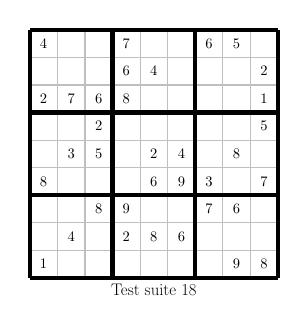
\begin{tikzpicture}[scale=\scale, every node/.style={scale=\scale}]
      \node[anchor=center,scale=1.5] at (0.5, 8.5) {$4$};
      \node[anchor=center,scale=1.5] at (3.5, 8.5) {$7$};
      \node[anchor=center,scale=1.5] at (6.5, 8.5) {$6$};
      \node[anchor=center,scale=1.5] at (7.5, 8.5) {$5$};
      \node[anchor=center,scale=1.5] at (3.5, 7.5) {$6$};
      \node[anchor=center,scale=1.5] at (4.5, 7.5) {$4$};
      \node[anchor=center,scale=1.5] at (8.5, 7.5) {$2$};
      \node[anchor=center,scale=1.5] at (0.5, 6.5) {$2$};
      \node[anchor=center,scale=1.5] at (1.5, 6.5) {$7$};
      \node[anchor=center,scale=1.5] at (2.5, 6.5) {$6$};
      \node[anchor=center,scale=1.5] at (3.5, 6.5) {$8$};
      \node[anchor=center,scale=1.5] at (8.5, 6.5) {$1$};
      \node[anchor=center,scale=1.5] at (2.5, 5.5) {$2$};
      \node[anchor=center,scale=1.5] at (8.5, 5.5) {$5$};
      \node[anchor=center,scale=1.5] at (1.5, 4.5) {$3$};
      \node[anchor=center,scale=1.5] at (2.5, 4.5) {$5$};
      \node[anchor=center,scale=1.5] at (4.5, 4.5) {$2$};
      \node[anchor=center,scale=1.5] at (5.5, 4.5) {$4$};
      \node[anchor=center,scale=1.5] at (7.5, 4.5) {$8$};
      \node[anchor=center,scale=1.5] at (0.5, 3.5) {$8$};
      \node[anchor=center,scale=1.5] at (4.5, 3.5) {$6$};
      \node[anchor=center,scale=1.5] at (5.5, 3.5) {$9$};
      \node[anchor=center,scale=1.5] at (6.5, 3.5) {$3$};
      \node[anchor=center,scale=1.5] at (8.5, 3.5) {$7$};
      \node[anchor=center,scale=1.5] at (2.5, 2.5) {$8$};
      \node[anchor=center,scale=1.5] at (3.5, 2.5) {$9$};
      \node[anchor=center,scale=1.5] at (6.5, 2.5) {$7$};
      \node[anchor=center,scale=1.5] at (7.5, 2.5) {$6$};
      \node[anchor=center,scale=1.5] at (1.5, 1.5) {$4$};
      \node[anchor=center,scale=1.5] at (3.5, 1.5) {$2$};
      \node[anchor=center,scale=1.5] at (4.5, 1.5) {$8$};
      \node[anchor=center,scale=1.5] at (5.5, 1.5) {$6$};
      \node[anchor=center,scale=1.5] at (0.5, 0.5) {$1$};
      \node[anchor=center,scale=1.5] at (7.5, 0.5) {$9$};
      \node[anchor=center,scale=1.5] at (8.5, 0.5) {$8$};
      \draw[gray!50] (0,0) grid (9,9);
      \draw[line width=0.55mm, scale=3] (0, 0) grid (3, 3);
      \draw (4.5,-.1) node[below] {\LARGE{Test suite 18}};
    \end{tikzpicture}
    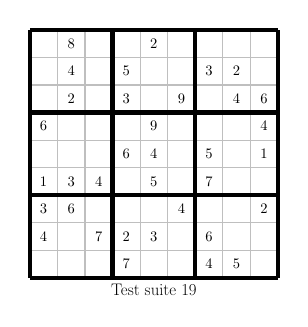
\begin{tikzpicture}[scale=\scale, every node/.style={scale=\scale}]
      \node[anchor=center,scale=1.5] at (1.5, 8.5) {$8$};
      \node[anchor=center,scale=1.5] at (4.5, 8.5) {$2$};
      \node[anchor=center,scale=1.5] at (1.5, 7.5) {$4$};
      \node[anchor=center,scale=1.5] at (3.5, 7.5) {$5$};
      \node[anchor=center,scale=1.5] at (6.5, 7.5) {$3$};
      \node[anchor=center,scale=1.5] at (7.5, 7.5) {$2$};
      \node[anchor=center,scale=1.5] at (1.5, 6.5) {$2$};
      \node[anchor=center,scale=1.5] at (3.5, 6.5) {$3$};
      \node[anchor=center,scale=1.5] at (5.5, 6.5) {$9$};
      \node[anchor=center,scale=1.5] at (7.5, 6.5) {$4$};
      \node[anchor=center,scale=1.5] at (8.5, 6.5) {$6$};
      \node[anchor=center,scale=1.5] at (0.5, 5.5) {$6$};
      \node[anchor=center,scale=1.5] at (4.5, 5.5) {$9$};
      \node[anchor=center,scale=1.5] at (8.5, 5.5) {$4$};
      \node[anchor=center,scale=1.5] at (3.5, 4.5) {$6$};
      \node[anchor=center,scale=1.5] at (4.5, 4.5) {$4$};
      \node[anchor=center,scale=1.5] at (6.5, 4.5) {$5$};
      \node[anchor=center,scale=1.5] at (8.5, 4.5) {$1$};
      \node[anchor=center,scale=1.5] at (0.5, 3.5) {$1$};
      \node[anchor=center,scale=1.5] at (1.5, 3.5) {$3$};
      \node[anchor=center,scale=1.5] at (2.5, 3.5) {$4$};
      \node[anchor=center,scale=1.5] at (4.5, 3.5) {$5$};
      \node[anchor=center,scale=1.5] at (6.5, 3.5) {$7$};
      \node[anchor=center,scale=1.5] at (0.5, 2.5) {$3$};
      \node[anchor=center,scale=1.5] at (1.5, 2.5) {$6$};
      \node[anchor=center,scale=1.5] at (5.5, 2.5) {$4$};
      \node[anchor=center,scale=1.5] at (8.5, 2.5) {$2$};
      \node[anchor=center,scale=1.5] at (0.5, 1.5) {$4$};
      \node[anchor=center,scale=1.5] at (2.5, 1.5) {$7$};
      \node[anchor=center,scale=1.5] at (3.5, 1.5) {$2$};
      \node[anchor=center,scale=1.5] at (4.5, 1.5) {$3$};
      \node[anchor=center,scale=1.5] at (6.5, 1.5) {$6$};
      \node[anchor=center,scale=1.5] at (3.5, 0.5) {$7$};
      \node[anchor=center,scale=1.5] at (6.5, 0.5) {$4$};
      \node[anchor=center,scale=1.5] at (7.5, 0.5) {$5$};
      \draw[gray!50] (0,0) grid (9,9);
      \draw[line width=0.55mm, scale=3] (0, 0) grid (3, 3);
      \draw (4.5,-.1) node[below] {\LARGE{Test suite 19}};
    \end{tikzpicture}
    
    
      \caption{All puzzles in the provided test suite.}
    \label{fig:exp1}
    \end{figure}
\end{center}

\begin{center}
  \begin{table}[H]
    \centering
    
    \rowcolors{2}{white}{gray!25}
    \resizebox{\columnwidth}{!}{%
    \begin{tabular}{crrrrrr}
      \cellcolor[gray]{0.7} & \multicolumn{2}{c}{BT\cellcolor[gray]{0.7}} & \multicolumn{2}{c}{BJ\cellcolor[gray]{0.7}}  & \multicolumn{2}{c}{CBJ\cellcolor[gray]{0.7}} \\
      \cellcolor[gray]{0.7} Test suite & \multicolumn{1}{c}{\cellcolor[gray]{0.7}Nodes} & \multicolumn{1}{c}{\cellcolor[gray]{0.7}Time(s)} & \multicolumn{1}{c}{\cellcolor[gray]{0.7}Nodes} & \multicolumn{1}{c}{\cellcolor[gray]{0.7}Time(s)} & \multicolumn{1}{c}{\cellcolor[gray]{0.7}Nodes} & \multicolumn{1}{c}{\cellcolor[gray]{0.7}Time(s)} \\
      0 & 10352 & 0.3891 & 1476 & 0.0707 & 1014 & 0.0345\\
      1 & 95775 & 4.0698 & 1863 & 0.051 & 1811 & 0.0456\\
      2 & 185358 & 8.3867 & 1375 & 0.0587 & 1103 & 0.0441\\
      3 & 210448 & 7.7151 & 27264 & 0.9803 & 16792 & 0.5794\\
      4 & 228100 & 7.2007 & 14753 & 0.4094 & 13557 & 0.3429\\
      5 & 274480 & 9.5221 & 41637 & 1.3549 & 22049 & 0.6689\\
      6 & 284079 & 8.3254 & 5084 & 0.117 & 3869 & 0.0861\\
      7 & 302346 & 12.7633 & 16895 & 0.7814 & 14021 & 0.5497\\
      8 & 339699 & 24.4524 & 3413 & 0.2283 & 3023 & 0.1789\\
      9 & 372341 & 16.7888 & 25137 & 1.27 & 14833 & 0.6722\\
      10 & 486884 & 35.5491 & 7005 & 0.3473 & 6525 & 0.3178\\
      11 & 1123918 & 64.8931 & 37668 & 1.918 & 32282 & 1.4768\\
      12 & 1181914 & 58.1829 & 15281 & 0.5672 & 12757 & 0.4258\\
      13 & 1247724 & 54.9106 & 87518 & 3.4041 & 24473 & 0.9547\\
      14 & 1962926 & 79.79 & 87572 & 3.2575 & 69020 & 2.3439\\
      15 & 2320445 & 112.1436 & 75454 & 2.9944 & 29344 & 1.1991\\
      16 & 2744246 & 86.076 & 122345 & 3.672 & 37604 & 1.7481\\
      17 & 3494453 & 165.2988 & 272558 & 10.2189 & 116351 & 4.2637\\
      18 & 8370963 & 503.3993 & 29105 & 1.2658 & 21899 & 0.9765\\
      19 & 12632761 & 605.4648 & 27060 & 0.8237 & 24086 & 0.7206\\
    \end{tabular}
    \rowcolors{2}{white}{gray!25}
    \begin{tabular}{crrrrrr}
      \cellcolor[gray]{0.7} & \multicolumn{2}{c}{BT\cellcolor[gray]{0.7}} & \multicolumn{2}{c}{BJ\cellcolor[gray]{0.7}}  & \multicolumn{2}{c}{CBJ\cellcolor[gray]{0.7}} \\
      \cellcolor[gray]{0.7} Test suite & \multicolumn{1}{c}{\cellcolor[gray]{0.7}Nodes} & \multicolumn{1}{c}{\cellcolor[gray]{0.7}Time(s)} & \multicolumn{1}{c}{\cellcolor[gray]{0.7}Nodes} & \multicolumn{1}{c}{\cellcolor[gray]{0.7}Time(s)} & \multicolumn{1}{c}{\cellcolor[gray]{0.7}Nodes} & \multicolumn{1}{c}{\cellcolor[gray]{0.7}Time(s)}\\
      0 & 81 & 0.0019 & 81 & 0.0029 & 81 & 0.0025\\
      1 & 81 & 0.002 & 81 & 0.0021 & 81 & 0.0029\\
      2 & 81 & 0.0027 & 81 & 0.0021 & 81 & 0.0099\\
      3 & 81 & 0.0025 & 81 & 0.0059 & 81 & 0.0036\\
      4 & 81 & 0.0026 & 81 & 0.0037 & 81 & 0.0049\\
      5 & 81 & 0.0042 & 81 & 0.0042 & 81 & 0.004\\
      6 & 81 & 0.0046 & 81 & 0.0066 & 81 & 0.0046\\
      7 & 81 & 0.004 & 81 & 0.0021 & 81 & 0.0024\\
      8 & 81 & 0.0033 & 81 & 0.0029 & 81 & 0.0036\\
      9 & 81 & 0.0022 & 81 & 0.0038 & 81 & 0.0035\\
      10 & 81 & 0.0044 & 81 & 0.0033 & 81 & 0.0035\\
      11 & 427 & 0.0119 & 353 & 0.0103 & 316 & 0.0097\\
      12 & 81 & 0.0022 & 81 & 0.0031 & 81 & 0.0028\\
      13 & 81 & 0.0023 & 81 & 0.0019 & 81 & 0.0045\\
      14 & 81 & 0.0023 & 81 & 0.0021 & 81 & 0.0022\\
      15 & 81 & 0.0024 & 81 & 0.0024 & 81 & 0.0023\\
      16 & 81 & 0.0026 & 81 & 0.0023 & 81 & 0.0031\\
      17 & 81 & 0.0093 & 81 & 0.0028 & 81 & 0.0076\\
      18 & 81 & 0.0028 & 81 & 0.0031 & 81 & 0.0021\\
      19 & 81 & 0.0051 & 81 & 0.0022 & 81 & 0.0025\\
    \end{tabular}
    }
    \caption{Performance of all three algorithms on the test suites without and with arc-consistency.}
    \label{tab:exp1}
  \end{table}
\end{center}

It is of no surprise that the performance increases as we become smarter with backtracking. Backjumping is an improvement on backtracking and conflict-directed backjumping is an improvement on backjumping. The most surprising results is probably that sometimes runs with less nodes expanded can take longer. This could be due to luck (or lack thereof) when checking constraints. As we stated earlier, each cell has 20 peers and in one run we could find the conflicting ones early on average while late in another.

Sudoku puzzles are often rated as easy or hard. These ratings do not necessarily translate to the algorithms we have implemented, i.e. an ``easy'' puzzle can be hard for a backtracking algorithm. In fact, puzzles can be designed to be hard for backtracking. The more assigned values the puzzle has, the easier - this most algorithms (and humans) can agree on. Another criteria for easiness is how many new assignments can be concluded by simple logic. That would however not make the problem any easier for backtracking algorithms, unless we preprocess the domains.

\begin{center}
  \begin{figure}[ht]
    \centering
    \def\scale{.35} % scale everything
    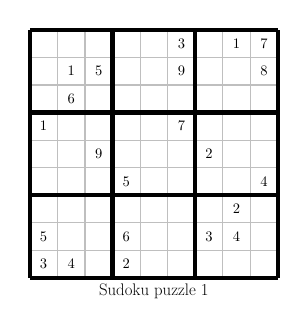
\begin{tikzpicture}[scale=\scale, every node/.style={scale=\scale}]
      \node[anchor=center,scale=1.5] at (5.5, 8.5) {$3$};
      \node[anchor=center,scale=1.5] at (7.5, 8.5) {$1$};
      \node[anchor=center,scale=1.5] at (8.5, 8.5) {$7$};
      \node[anchor=center,scale=1.5] at (1.5, 7.5) {$1$};
      \node[anchor=center,scale=1.5] at (2.5, 7.5) {$5$};
      \node[anchor=center,scale=1.5] at (5.5, 7.5) {$9$};
      \node[anchor=center,scale=1.5] at (8.5, 7.5) {$8$};
      \node[anchor=center,scale=1.5] at (1.5, 6.5) {$6$};
      \node[anchor=center,scale=1.5] at (0.5, 5.5) {$1$};
      \node[anchor=center,scale=1.5] at (5.5, 5.5) {$7$};
      \node[anchor=center,scale=1.5] at (2.5, 4.5) {$9$};
      \node[anchor=center,scale=1.5] at (6.5, 4.5) {$2$};
      \node[anchor=center,scale=1.5] at (3.5, 3.5) {$5$};
      \node[anchor=center,scale=1.5] at (8.5, 3.5) {$4$};
      \node[anchor=center,scale=1.5] at (7.5, 2.5) {$2$};
      \node[anchor=center,scale=1.5] at (0.5, 1.5) {$5$};
      \node[anchor=center,scale=1.5] at (3.5, 1.5) {$6$};
      \node[anchor=center,scale=1.5] at (6.5, 1.5) {$3$};
      \node[anchor=center,scale=1.5] at (7.5, 1.5) {$4$};
      \node[anchor=center,scale=1.5] at (0.5, 0.5) {$3$};
      \node[anchor=center,scale=1.5] at (1.5, 0.5) {$4$};
      \node[anchor=center,scale=1.5] at (3.5, 0.5) {$2$};
      \draw[gray!50] (0,0) grid (9,9);
      \draw[line width=0.55mm, scale=3] (0, 0) grid (3, 3);
      \draw (4.5,-.1) node[below] {\LARGE{Sudoku puzzle 1}};
    \end{tikzpicture}
    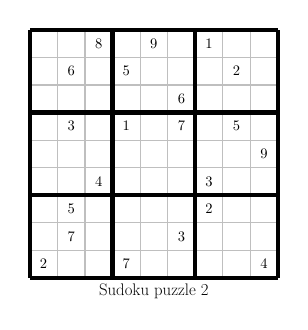
\begin{tikzpicture}[scale=\scale, every node/.style={scale=\scale}]
      \node[anchor=center,scale=1.5] at (2.5, 8.5) {$8$};
      \node[anchor=center,scale=1.5] at (4.5, 8.5) {$9$};
      \node[anchor=center,scale=1.5] at (6.5, 8.5) {$1$};
      \node[anchor=center,scale=1.5] at (1.5, 7.5) {$6$};
      \node[anchor=center,scale=1.5] at (3.5, 7.5) {$5$};
      \node[anchor=center,scale=1.5] at (7.5, 7.5) {$2$};
      \node[anchor=center,scale=1.5] at (5.5, 6.5) {$6$};
      \node[anchor=center,scale=1.5] at (1.5, 5.5) {$3$};
      \node[anchor=center,scale=1.5] at (3.5, 5.5) {$1$};
      \node[anchor=center,scale=1.5] at (5.5, 5.5) {$7$};
      \node[anchor=center,scale=1.5] at (7.5, 5.5) {$5$};
      \node[anchor=center,scale=1.5] at (8.5, 4.5) {$9$};
      \node[anchor=center,scale=1.5] at (2.5, 3.5) {$4$};
      \node[anchor=center,scale=1.5] at (6.5, 3.5) {$3$};
      \node[anchor=center,scale=1.5] at (1.5, 2.5) {$5$};
      \node[anchor=center,scale=1.5] at (6.5, 2.5) {$2$};
      \node[anchor=center,scale=1.5] at (1.5, 1.5) {$7$};
      \node[anchor=center,scale=1.5] at (5.5, 1.5) {$3$};
      \node[anchor=center,scale=1.5] at (0.5, 0.5) {$2$};
      \node[anchor=center,scale=1.5] at (3.5, 0.5) {$7$};
      \node[anchor=center,scale=1.5] at (8.5, 0.5) {$4$};
      \draw[gray!50] (0,0) grid (9,9);
      \draw[line width=0.55mm, scale=3] (0, 0) grid (3, 3);
      \draw (4.5,-.1) node[below] {\LARGE{Sudoku puzzle 2}};
    \end{tikzpicture}
    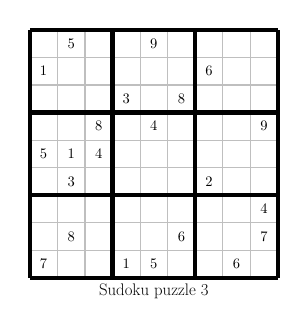
\begin{tikzpicture}[scale=\scale, every node/.style={scale=\scale}]
      \node[anchor=center,scale=1.5] at (1.5, 8.5) {$5$};
      \node[anchor=center,scale=1.5] at (4.5, 8.5) {$9$};
      \node[anchor=center,scale=1.5] at (0.5, 7.5) {$1$};
      \node[anchor=center,scale=1.5] at (6.5, 7.5) {$6$};
      \node[anchor=center,scale=1.5] at (3.5, 6.5) {$3$};
      \node[anchor=center,scale=1.5] at (5.5, 6.5) {$8$};
      \node[anchor=center,scale=1.5] at (2.5, 5.5) {$8$};
      \node[anchor=center,scale=1.5] at (4.5, 5.5) {$4$};
      \node[anchor=center,scale=1.5] at (8.5, 5.5) {$9$};
      \node[anchor=center,scale=1.5] at (0.5, 4.5) {$5$};
      \node[anchor=center,scale=1.5] at (1.5, 4.5) {$1$};
      \node[anchor=center,scale=1.5] at (2.5, 4.5) {$4$};
      \node[anchor=center,scale=1.5] at (1.5, 3.5) {$3$};
      \node[anchor=center,scale=1.5] at (6.5, 3.5) {$2$};
      \node[anchor=center,scale=1.5] at (8.5, 2.5) {$4$};
      \node[anchor=center,scale=1.5] at (1.5, 1.5) {$8$};
      \node[anchor=center,scale=1.5] at (5.5, 1.5) {$6$};
      \node[anchor=center,scale=1.5] at (8.5, 1.5) {$7$};
      \node[anchor=center,scale=1.5] at (0.5, 0.5) {$7$};
      \node[anchor=center,scale=1.5] at (3.5, 0.5) {$1$};
      \node[anchor=center,scale=1.5] at (4.5, 0.5) {$5$};
      \node[anchor=center,scale=1.5] at (7.5, 0.5) {$6$};
      \draw[gray!50] (0,0) grid (9,9);
      \draw[line width=0.55mm, scale=3] (0, 0) grid (3, 3);
      \draw (4.5,-.1) node[below] {\LARGE{Sudoku puzzle 3}};
    \end{tikzpicture}
    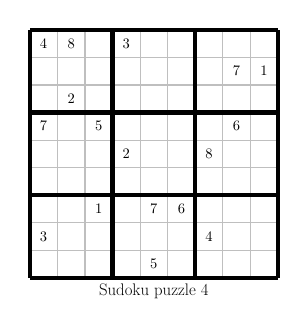
\begin{tikzpicture}[scale=\scale, every node/.style={scale=\scale}]
      \node[anchor=center,scale=1.5] at (0.5, 8.5) {$4$};
      \node[anchor=center,scale=1.5] at (1.5, 8.5) {$8$};
      \node[anchor=center,scale=1.5] at (3.5, 8.5) {$3$};
      \node[anchor=center,scale=1.5] at (7.5, 7.5) {$7$};
      \node[anchor=center,scale=1.5] at (8.5, 7.5) {$1$};
      \node[anchor=center,scale=1.5] at (1.5, 6.5) {$2$};
      \node[anchor=center,scale=1.5] at (0.5, 5.5) {$7$};
      \node[anchor=center,scale=1.5] at (2.5, 5.5) {$5$};
      \node[anchor=center,scale=1.5] at (7.5, 5.5) {$6$};
      \node[anchor=center,scale=1.5] at (3.5, 4.5) {$2$};
      \node[anchor=center,scale=1.5] at (6.5, 4.5) {$8$};
      \node[anchor=center,scale=1.5] at (2.5, 2.5) {$1$};
      \node[anchor=center,scale=1.5] at (4.5, 2.5) {$7$};
      \node[anchor=center,scale=1.5] at (5.5, 2.5) {$6$};
      \node[anchor=center,scale=1.5] at (0.5, 1.5) {$3$};
      \node[anchor=center,scale=1.5] at (6.5, 1.5) {$4$};
      \node[anchor=center,scale=1.5] at (4.5, 0.5) {$5$};
      \draw[gray!50] (0,0) grid (9,9);
      \draw[line width=0.55mm, scale=3] (0, 0) grid (3, 3);
      \draw (4.5,-.1) node[below] {\LARGE{Sudoku puzzle 4}};
    \end{tikzpicture}
    \caption{The additional Sudoku puzzles used for experiments with arc-consistency.}
    \label{fig:exp3}
  \end{figure}
\end{center}

When the test suites were run with arc-consistency, only one was not solved directly by it and that was test suite 11. It required 427, 353 and 316 nodes to be expanded for backtracking, backjumping and conflict-directed backjumping respectively and all 20 test suites were solved within $0.012$ seconds by all algorithms. With such a minuscule difference in performance, we needed different puzzles to compare the algorithms with arc-consistency. We chose 4 puzzles from the additional puzzles provided and ran the three algorithms for all of them. The puzzle we chose can be seen in Figure \ref{fig:exp3}. The performance of our algorithms can be seen in Table \ref{tab:exp3}. Like before, the algorithms that are built as improvements outperform their prototypes, as is expected.

\begin{center}     
  \begin{table}[ht]
    \centering
    \rowcolors{2}{white}{gray!25}
    
    \begin{tabular}{crrrrrr}
      \cellcolor[gray]{0.7} & \multicolumn{2}{c}{BT\cellcolor[gray]{0.7}} & \multicolumn{2}{c}{BJ\cellcolor[gray]{0.7}}  & \multicolumn{2}{c}{CBJ\cellcolor[gray]{0.7}} \\
      \cellcolor[gray]{0.7} Sudoku puzzle & \multicolumn{1}{c}{\cellcolor[gray]{0.7}Nodes} & \multicolumn{1}{c}{\cellcolor[gray]{0.7}Time(s)} & \multicolumn{1}{c}{\cellcolor[gray]{0.7}Nodes} & \multicolumn{1}{c}{\cellcolor[gray]{0.7}Time(s)} & \multicolumn{1}{c}{\cellcolor[gray]{0.7}Nodes} & \multicolumn{1}{c}{\cellcolor[gray]{0.7}Time(s)} \\
      1 & 2339 & 0.1174 & 1652 & 0.0741 & 764 & 0.03\\
      2 & 160054 & 9.5492 & 90200 & 3.529 & 54765 & 1.734\\
      3 & 540279 & 25.149 & 353457 & 13.6457 & 152490 & 5.3534\\
      4 & 478270 & 30.9214 & 340839 & 17.3177 & 189604 & 8.8046\\
    \end{tabular}
    \caption{Performance of all three algorithms on the additional puzzles with arc-consistency.}
    \label{tab:exp3}
  \end{table}
\end{center}